\chapter{Software structure and optional modules}\label{ChapSoftwareStructure}
Ash3d has been under development since 2009 and has evolved to suit
the needs of both operational forecasting as well as a research tool.
As research ideas were tested and bits of code were altered and inserted
at various points in the software, this evolution lead to dormant
branches of the code, inefficiencies, changes in default values that became
part of the operational branch, and occasionally the introduction of 
bugs in the code.  To mitigate these problems and to facilitate the
development of new features or research ideas without affecting the core
functionality of the software, we began an effort to re-structure the
software.  The restructuring has been guided by several goals:
to group and isolate common-themed functions and variables into modules,
to separate reusable code into libraries,
to optimize structure of and access to the main variables,
to isolate essential functionality into a core set of subroutines that
would require minimal continued development, and
to move all the essential control structure of the program to 
the top-level file (\texttt{Ash3d.F90}).
This software structure would be a minimal `core code' to be available for
operational usage or for research efforts requiring only essential functionality.
If a non-essential feature were needed to address a question (e.g. predicting
the resuspension of deposited ash, tracking the advection of fallout with
ocean surface currents), then this feature could be isolated in an optional
module which could be compiled with a version of the \texttt{Ash3d.F90} linking
to all the core-code files.

The structure of the core code is outlined in Figure \ref{FigSoftwareDesign}.
The files are broadly sorted into those needed for setup/initialization,
calculation of meteorological values, source terms, advection routines, 
diffusion routines, and output.  Files that define modules are encircled
by bold lines.  Files that need direct access to the main array of concentration
values (\texttt{concen\_pd}) are colored orange.  The number of files with
access to \texttt{concen\_pd} is minimized since repeated access to this
array can effect performance, particularly on hybrid GPU/CPU systems.
\begin{figure}[htbp]\begin{center}
 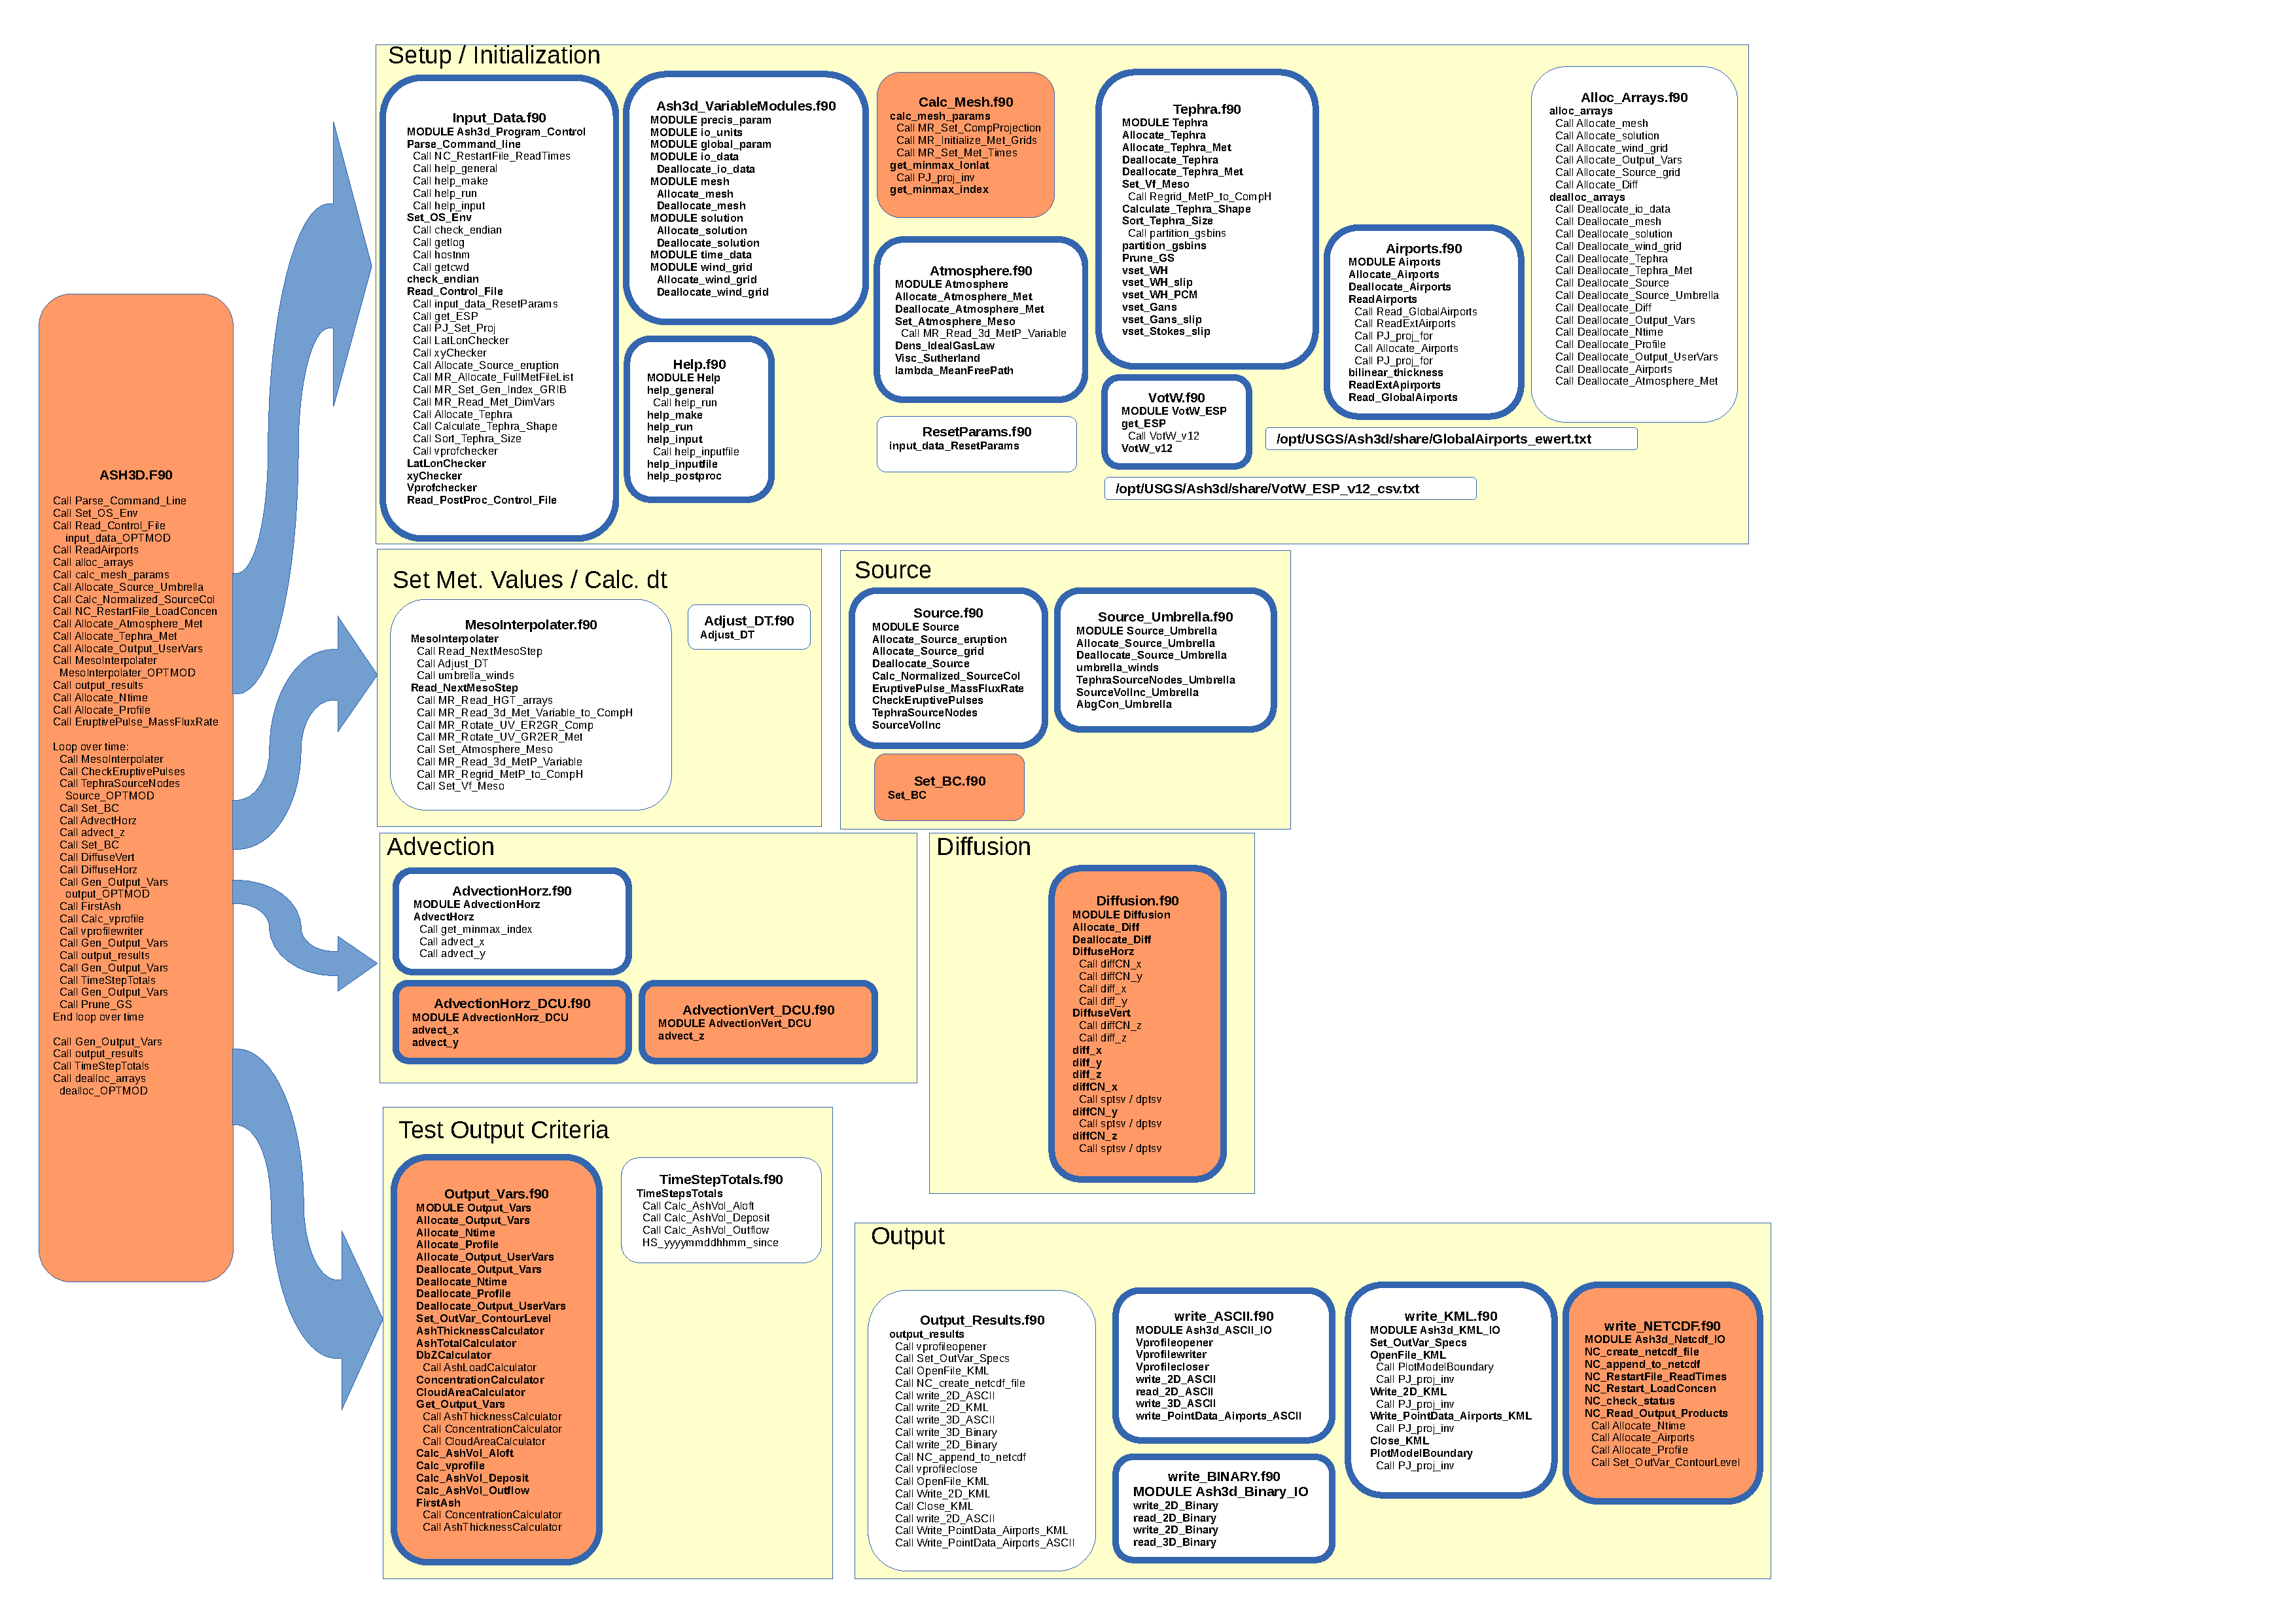
\includegraphics[angle=90,scale=0.35]{Figures/Chap_SoftStruct_FlowChartFiles.pdf}
\parbox{15cm}{\caption{\label{FigSoftwareDesign}
Ash3d program structure.
}}
\end{center}\end{figure}

The basic flow of the code is as follows:
\begin{enumerate}
 \item Initialize Run
 \begin{itemize}
  \item[$-$] Test runtime environment (variables, OpenMP, test system configuration)
  \item[$-$] Parse command-line / read control file
  \item[$-$] Read auxiliary data: airport/POI and volcano lists
  \item[$-$] Calculate computational mesh parameters
  \item[$-$] Allocate memory
  \item[$-$] Initialize concentration array (possibly with source)
  \item[$-$] Read meteorological files for starting values
  \item[$-$] Initialize output files
 \end{itemize}
 \item Solve advection-diffusion equations
 \begin{itemize}
  \item[$-$] Start time loop
  \item[$-$] Update atmospheric data for current time
  \item[$-$] Calculate source term
  \item[$-$] Set boundary conditions
  \item[$-$] Advect horizontally
  \item[$-$] Advect vertically
  \item[$-$] Diffuse vertically
  \item[$-$] Diffuse horizontally
  \item[$-$] Test for output criteria (log-step, output step)
  \item[$-$] Write output data if needed
  \item[$-$] Check stop conditions (end time reached, no ash aloft, etc.)
  \item[$-$] Integrate solution forward in time
 \end{itemize}
 \item Closing routines
 \begin{itemize}
  \item[$-$] Finalize output
  \item[$-$] Deallocate all memory
 \end{itemize}
\end{enumerate}


%%%%%%%%%%%%%%%%%%%%%%%%%%%%%%%%%%%%%%%%%%%%%%%%%%%%%%%%%%%%%%%%%%%%%%%%%%%%%%%
\section{User-customization}\label{ChapSoftwareStructureUserCust}
Although Ash3d is not a particularly large program, understanding all the
details of the software is a cumbersome and largely unnecessary task.  In
order to modify Ash3d to include a new feature (source term,
evolution or removal mechanism, etc.), the recommended approach is to
create the new routines in a separate module and edit a copy of the main
program file \texttt{Ash3d.F90} to include calls to these routines.  The makefile
can be edited to build this new module and link with the objects in the
core-code repository.  \texttt{Ash3d.F90} has commented sections throughout
that indicate where edits would be needed to link to the new module.

An example
of using an optional module is given in the git repository
\url{https://github.com/usgs/hschwaiger-usgs/Ash3d\_OptionalModules}.
The makefile in this repository contains the variable
\texttt{ASH3dCCSRC=/work/USGS/Software\_repos/GIT/Ash3d/src} which points to the
location of the Ash3d source files.  The optional module included in this repository
is for running the various test cases to test the convergence properties
of the code (see Section \ref{ApxTestSecConv}).  The main program file is replaced with
\texttt{Ash3d\_TC.F90} which contain all the function calls needed to set up and
run the test cases.  In this example, the additional code is invoked using
pre-processor directives, though this is not necessary.
This module is not especially invasive and only requires a few subroutine calls:
a call to \texttt{set\_TestCase\_globvars} which sets global variables turning on/off
advection and diffusion routines, a call to \texttt{set\_TestCase\_windfield} and
\texttt{DistSource} to specify the wind field and initialize the source, a disabling
of \texttt{MassFluxCalculator}, and finally a call to \texttt{Testcase\_CalcErrors}
which prepares the output data. The goal is to have all additional subroutine callable
from the top level file (\texttt{Ash3d\_TC.F90}) with all others linked to
the core repository of the Ash3d
code. In this example, \texttt{Set\_BC.f90} needed to be modified for the
test case using the Method of Manufactured Solution as is replaced with
\texttt{Set\_BC\_TC.f90}.
Details of this module along with instructions on running the scripts can be found
in Appendix \ref{ChapAppendTestCases}.

For a more general case, an example is given for the module for the accelerated
removal mechanisms of ash due to hydrometeors (e.g. wet deposition).  As before,
the only files that need to be modified from the core-code Ash3d version is the
top-level file (a copy of \texttt{Ash3d.F90} and the \texttt{makefile}.  Additionally,
the module containing all the public variables and routines is needed.  There are
several subroutines that are generally needed.  Firstly, if a dedicated block of
the input file is to be read for module-specific input values, a subroutine such
as \texttt{input\_data\_WetDepo} should be included.

\small
\begin{verbatim}
        ! input data for ash transport
      call Read_Control_File
!------------------------------------------------------------------------------
!       OPTIONAL MODULES
!         Insert calls to custom input blocks here

      write(global_info,*)&
        "Now looping through optional modules found in input file"
      do j=1,nmods
        write(global_info,*)"Testing for ",OPTMOD_names(j),j
#ifdef WETDEPO
        if(OPTMOD_names(j).eq.'WETDEPO')then
          write(global_info,*)"  Reading input block for WETDEPO"
          call input_data_WetDepo
        endif
#endif
!
!------------------------------------------------------------------------------
\end{verbatim}
\normalsize
The structure of this optional module block can be designed to the user's needs
and can have as many lines as necessary to fully characterize all the necessary
parameters. In this case, for example, we might want have fields to enable or
disable different removal mechanisms via hydrometeors (rain scavenging, cloud
condensation nucleation, etc.). These mechanisms might have parameters associated
with scavenging rate or a different fall mechanics. Maybe there are specialize
output variables that might optionally be included in the output file that could
be toggled on or off via settings in this block.

%\small  
%\begin{verbatim}
%!------------------------------------------------------------------------------
%!       OPTIONAL MODULES
%!         Insert special source terms here
%!
%#ifdef SRC_SAT
%      if(SourceType.eq.'satellite')then
%        ! Satellite initialized runs have a concen array loaded here
%        call Allocate_Source_Satellite
%        call Read_SatMassLoading
%      endif
%#endif
%!------------------------------------------------------------------------------
%\end{verbatim}
%\normalsize

%Output_Vars
%var_User2d_static_XY
%var_User2d_XY
%var_User3d_XYGs
%var_User3d_XYZ
%var_User4d_XYZGs

Next, the space needed for storing module-specific variables (some on the 
computational grid and some only on the meteorological grid) needs to be
allocated.  
\small
\begin{verbatim}
!------------------------------------------------------------------------------
!       OPTIONAL MODULES
!         Insert calls to optional variable allocation subroutines here
!
#ifdef WETDEPO
      if(USE_WETDEPO)then
        call Allocate_WetDepo_global
        call Allocate_WetDepo_Met
      endif
#endif
\end{verbatim}
\normalsize
In principle, the variables on the meteorological grid and on the computational
grid could be allocated in the same subroutine, but we generally separate them
for clarity.

If any of the calculations rely on fields read from the numerical weather
prediction files, then we need a subroutine to read and interpolate these
data.  The list of variables available to read is given in Table 1 of Appendix 8.1
of the MetReader documentation.
\small
\begin{verbatim}
!------------------------------------------------------------------------------
!       OPTIONAL MODULES
!         Insert calls to special MesoInterpolaters subroutines here
!
#ifdef WETDEPO
        if(USE_WETDEPO)     call Set_WetDepo_Meso(Load_MesoSteps,Interval_Frac)
#endif
\end{verbatim}
\normalsize
For example, the scavenging of particles from the atmosphere is dependent on
the precipitation rate (variable code \texttt{44} from the MetReader documentation).
So to calculate the scavenging coefficient at each time-step, one would read the
precipitation rate for the bracketing NWP time steps, interpolate to the computational
grid, then calculate the scavenging coefficients on the computational grid at the
meteorological time steps, then finally interpolating to the current time:
\small
\begin{verbatim}
ivar = 44 !  Precipitation rate large-scale (liquid)
call MR_Read_2d_Met_Variable(ivar,MR_iMetStep_Now)
call MR_Regrid_MetP_to_CompGrid(MR_iMetStep_Now)
precipitation_rate_2d(:,:)   = MR_dum2d_comp(:,:)
call Set_Scav_Coeff(MR_iMetStep_Now,1)

call MR_Read_2d_Met_Variable(ivar,MR_iMetStep_Now+1)
call MR_Regrid_MetP_to_CompGrid(MR_iMetStep_Now+1)
precipitation_rate_2d(:,:)   = MR_dum2d_comp(:,:)
call Set_Scav_Coeff(MR_iMetStep_Now+1,2)

call Interpolate_WetDepo(Interval_Frac)
\end{verbatim}
\normalsize
If any variables are needed for output to the NetCDF file, the list of output
variables in the module \texttt{Output\_Vars} can be appended.  These variables
in \texttt{Output\_Vars} are sorted by their dimensionality:
\small
\begin{verbatim}
var_User2d_static_XY  ! 2d variable (nx,ny)
var_User2d_XY         ! 3d variably (nx,ny,nt)
var_User3d_XYGs       ! 4d variable (nx,ny,ns,nt)
var_User3d_XYZ        ! 4d variable (nx,ny,nz,nt)
var_User4d_XYZGs      ! 5d variable (nx,ny,nz,ns,nt
\end{verbatim}
\normalsize
A subroutine for preparing the master list of variables, their names, units,
FillValues, etc. should be called prior to the initialization of the output file.
For example, if only the 2-D surface precipitation and the 4-D scavenging coefficients
are added to the output file, the module should include:

\small
\begin{verbatim}
nvar_User2d_XY_WetDepo    = 1
nvar_User4d_XYZGs_WetDepo = 1
ivar = 1
temp_2d_name_WetDepo(ivar)  = "p0"
temp_2d_lname_WetDepo(ivar) = "Precipitation rate @ surf"
temp_2d_unit_WetDepo(ivar)  = "kg/m2/s"
temp_2d_MissVal_WetDepo(ivar) = -9999.0_op
temp_2d_FillVal_WetDepo(ivar) = -9999.0_op

ivar = 1
temp_4d_name_WetDepo(ivar)  = "ScavCo_liq"
temp_4d_lname_WetDepo(ivar) = "Scavenging coefficient"
temp_4d_unit_WetDepo(ivar)  = "1/hr"
temp_4d_MissVal_WetDepo(ivar) = -9999.0_op
temp_4d_FillVal_WetDepo(ivar) = -9999.0_op
nvar_User2d_XY    = nvar_User2d_XY        + nvar_User2d_XY_WetDepo
nvar_User4d_XYZGs = nvar_User4d_XYZGs     + nvar_User4d_XYZGs_WetDepo
\end{verbatim}
\normalsize

Then to actually update the master list of output variables in \texttt{Output\_Vars.f90},
use a subroutine such as:
\small
\begin{verbatim}
!------------------------------------------------------------------------------
!       OPTIONAL MODULES
!         Insert calls to prep user-specified output
!
#ifdef WETDEPO
      if(USE_WETDEPO) call Prep_output_WetDepo
#endif
\end{verbatim}
\normalsize
with code to update the master lists:
\small
\begin{verbatim}
do i=1,nvar_User4d_XYZGs_WetDepo
  indx = indx_User4d_XYZGs_WetDepo+i
  var_User4d_XYZGs_name(indx)   = temp_4d_name_WetDepo(i)
  var_User4d_XYZGs_unit(indx)   = temp_4d_unit_WetDepo(i)
  var_User4d_XYZGs_lname(indx)  = temp_4d_lname_WetDepo(i)
  var_User4d_XYZGs_MissVal(indx)= temp_4d_MissVal_WetDepo(i)
  var_User4d_XYZGs_FillVal(indx)= temp_4d_FillVal_WetDepo(i)
  if(i.eq.1) &
  var_User4d_XYZGs(1:nxmax,1:nymax,1:nzmax,1:n_gs_max,indx) = &
  real(scav_coeff_Liq_3d(1:nxmax,1:nymax,1:nzmax,1:n_gs_max),kind=op)
enddo
\end{verbatim}
\normalsize

After the start of the time loop, the interpolation routine that calculates
variables on the computational grid at the current time step from the NWP
files need to be called.
\small
\begin{verbatim}
          ! find the wind field at the current time
        first_time     = .false.
        call MesoInterpolater(time , Load_MesoSteps , Interval_Frac, first_time)
!------------------------------------------------------------------------------
!       OPTIONAL MODULES
!         Insert calls to special MesoInterpolaters subroutines here
!
#ifdef WETDEPO
        if(USE_WETDEPO)     call Set_WetDepo_Meso(Load_MesoSteps,Interval_Frac)
#endif
!------------------------------------------------------------------------------
\end{verbatim}
\normalsize

Within the time loop, any physics that effects the simulation can be called.
For the wet removal of airborne tephra, for example, a concentration-dependent
decay of the ash is calculated through sub-stepping (due to the stiffness of the
decay equations) over the full time step.
\small
\begin{verbatim}
!------------------------------------------------------------------------------
!       OPTIONAL MODULES
!         Insert calls to optional deposition routines here
!
#ifdef WETDEPO
        if(USE_WETDEPO)then
          call Wet_Depo_Rainout
        endif
#endif
!------------------------------------------------------------------------------
\end{verbatim}
\normalsize
Then, any output variables can be calculated with the corresponding
\texttt{var\_User2d\_[---]} variables updated. These will be written to the
NetCDF file, if that output format is specified in the Ash3d control file.

\small
\begin{verbatim}
!------------------------------------------------------------------------------
!       OPTIONAL MODULES
!         Insert calls output routines (every log-step) here
!
#ifdef WETDEPO
              if(USE_WETDEPO) call ThicknessCalculator_WetDepo
#endif
!------------------------------------------------------------------------------
\end{verbatim}
\normalsize
And finally after the completion of the time-step loop, routines for freeing
the allocated memory should be called.
\small
\begin{verbatim}
      ! clean up memory
      call dealloc_arrays
!------------------------------------------------------------------------------
!       OPTIONAL MODULES
!         Insert calls deallocation routines here
!
#ifdef WETDEPO
      if(USE_WETDEPO)then
        call Deallocate_WetDepo_global
        call Deallocate_WetDepo_Met
      endif
#endif
!------------------------------------------------------------------------------
\end{verbatim}
\normalsize

Except in unusual circumstances, these subroutine should be called from the
replaced top-level file, (e.g. \texttt{Ash3d\_WetDepo.F90}).

